% GNUPLOT: LaTeX picture with Postscript
\begingroup
  \makeatletter
  \providecommand\color[2][]{%
    \GenericError{(gnuplot) \space\space\space\@spaces}{%
      Package color not loaded in conjunction with
      terminal option `colourtext'%
    }{See the gnuplot documentation for explanation.%
    }{Either use 'blacktext' in gnuplot or load the package
      color.sty in LaTeX.}%
    \renewcommand\color[2][]{}%
  }%
  \providecommand\includegraphics[2][]{%
    \GenericError{(gnuplot) \space\space\space\@spaces}{%
      Package graphicx or graphics not loaded%
    }{See the gnuplot documentation for explanation.%
    }{The gnuplot epslatex terminal needs graphicx.sty or graphics.sty.}%
    \renewcommand\includegraphics[2][]{}%
  }%
  \providecommand\rotatebox[2]{#2}%
  \@ifundefined{ifGPcolor}{%
    \newif\ifGPcolor
    \GPcolortrue
  }{}%
  \@ifundefined{ifGPblacktext}{%
    \newif\ifGPblacktext
    \GPblacktextfalse
  }{}%
  % define a \g@addto@macro without @ in the name:
  \let\gplgaddtomacro\g@addto@macro
  % define empty templates for all commands taking text:
  \gdef\gplbacktext{}%
  \gdef\gplfronttext{}%
  \makeatother
  \ifGPblacktext
    % no textcolor at all
    \def\colorrgb#1{}%
    \def\colorgray#1{}%
  \else
    % gray or color?
    \ifGPcolor
      \def\colorrgb#1{\color[rgb]{#1}}%
      \def\colorgray#1{\color[gray]{#1}}%
      \expandafter\def\csname LTw\endcsname{\color{white}}%
      \expandafter\def\csname LTb\endcsname{\color{black}}%
      \expandafter\def\csname LTa\endcsname{\color{black}}%
      \expandafter\def\csname LT0\endcsname{\color[rgb]{1,0,0}}%
      \expandafter\def\csname LT1\endcsname{\color[rgb]{0,1,0}}%
      \expandafter\def\csname LT2\endcsname{\color[rgb]{0,0,1}}%
      \expandafter\def\csname LT3\endcsname{\color[rgb]{1,0,1}}%
      \expandafter\def\csname LT4\endcsname{\color[rgb]{0,1,1}}%
      \expandafter\def\csname LT5\endcsname{\color[rgb]{1,1,0}}%
      \expandafter\def\csname LT6\endcsname{\color[rgb]{0,0,0}}%
      \expandafter\def\csname LT7\endcsname{\color[rgb]{1,0.3,0}}%
      \expandafter\def\csname LT8\endcsname{\color[rgb]{0.5,0.5,0.5}}%
    \else
      % gray
      \def\colorrgb#1{\color{black}}%
      \def\colorgray#1{\color[gray]{#1}}%
      \expandafter\def\csname LTw\endcsname{\color{white}}%
      \expandafter\def\csname LTb\endcsname{\color{black}}%
      \expandafter\def\csname LTa\endcsname{\color{black}}%
      \expandafter\def\csname LT0\endcsname{\color{black}}%
      \expandafter\def\csname LT1\endcsname{\color{black}}%
      \expandafter\def\csname LT2\endcsname{\color{black}}%
      \expandafter\def\csname LT3\endcsname{\color{black}}%
      \expandafter\def\csname LT4\endcsname{\color{black}}%
      \expandafter\def\csname LT5\endcsname{\color{black}}%
      \expandafter\def\csname LT6\endcsname{\color{black}}%
      \expandafter\def\csname LT7\endcsname{\color{black}}%
      \expandafter\def\csname LT8\endcsname{\color{black}}%
    \fi
  \fi
    \setlength{\unitlength}{0.0500bp}%
    \ifx\gptboxheight\undefined%
      \newlength{\gptboxheight}%
      \newlength{\gptboxwidth}%
      \newsavebox{\gptboxtext}%
    \fi%
    \setlength{\fboxrule}{0.5pt}%
    \setlength{\fboxsep}{1pt}%
\begin{picture}(5100.00,9060.00)%
    \gplgaddtomacro\gplbacktext{%
      \csname LTb\endcsname%
      \put(534,6795){\makebox(0,0)[r]{\strut{}$0$}}%
      \csname LTb\endcsname%
      \put(534,7175){\makebox(0,0)[r]{\strut{}$0.2$}}%
      \csname LTb\endcsname%
      \put(534,7555){\makebox(0,0)[r]{\strut{}$0.4$}}%
      \csname LTb\endcsname%
      \put(534,7936){\makebox(0,0)[r]{\strut{}$0.6$}}%
      \csname LTb\endcsname%
      \put(534,8316){\makebox(0,0)[r]{\strut{}$0.8$}}%
      \csname LTb\endcsname%
      \put(534,8696){\makebox(0,0)[r]{\strut{}$1$}}%
      \csname LTb\endcsname%
      \put(623,6617){\makebox(0,0){\strut{}}}%
      \csname LTb\endcsname%
      \put(1465,6617){\makebox(0,0){\strut{}}}%
      \csname LTb\endcsname%
      \put(2307,6617){\makebox(0,0){\strut{}}}%
      \csname LTb\endcsname%
      \put(3148,6617){\makebox(0,0){\strut{}}}%
      \csname LTb\endcsname%
      \put(3990,6617){\makebox(0,0){\strut{}}}%
      \csname LTb\endcsname%
      \put(4832,6617){\makebox(0,0){\strut{}}}%
    }%
    \gplgaddtomacro\gplfronttext{%
      \csname LTb\endcsname%
      \put(89,7745){\rotatebox{-270}{\makebox(0,0){\strut{}\textbf{(a)} Interpolation $q$}}}%
      \csname LTb\endcsname%
      \put(2692,8900){\makebox(0,0)[r]{\strut{}$C\ix{high}$}}%
    }%
    \gplgaddtomacro\gplbacktext{%
      \csname LTb\endcsname%
      \put(534,4711){\makebox(0,0)[r]{\strut{}$0$}}%
      \csname LTb\endcsname%
      \put(534,5028){\makebox(0,0)[r]{\strut{}$5$}}%
      \csname LTb\endcsname%
      \put(534,5345){\makebox(0,0)[r]{\strut{}$10$}}%
      \csname LTb\endcsname%
      \put(534,5662){\makebox(0,0)[r]{\strut{}$15$}}%
      \csname LTb\endcsname%
      \put(534,5979){\makebox(0,0)[r]{\strut{}$20$}}%
      \csname LTb\endcsname%
      \put(534,6296){\makebox(0,0)[r]{\strut{}$25$}}%
      \csname LTb\endcsname%
      \put(534,6613){\makebox(0,0)[r]{\strut{}$30$}}%
      \csname LTb\endcsname%
      \put(623,4533){\makebox(0,0){\strut{}}}%
      \csname LTb\endcsname%
      \put(1465,4533){\makebox(0,0){\strut{}}}%
      \csname LTb\endcsname%
      \put(2307,4533){\makebox(0,0){\strut{}}}%
      \csname LTb\endcsname%
      \put(3148,4533){\makebox(0,0){\strut{}}}%
      \csname LTb\endcsname%
      \put(3990,4533){\makebox(0,0){\strut{}}}%
      \csname LTb\endcsname%
      \put(4832,4533){\makebox(0,0){\strut{}}}%
    }%
    \gplgaddtomacro\gplfronttext{%
      \csname LTb\endcsname%
      \put(178,5662){\rotatebox{-270}{\makebox(0,0){\strut{}\textbf{(b)} Probability $\ERprob$}}}%
    }%
    \gplgaddtomacro\gplbacktext{%
      \csname LTb\endcsname%
      \put(534,2627){\makebox(0,0)[r]{\strut{}$0$}}%
      \csname LTb\endcsname%
      \put(534,2817){\makebox(0,0)[r]{\strut{}$0.5$}}%
      \csname LTb\endcsname%
      \put(534,3007){\makebox(0,0)[r]{\strut{}$1$}}%
      \csname LTb\endcsname%
      \put(534,3198){\makebox(0,0)[r]{\strut{}$1.5$}}%
      \csname LTb\endcsname%
      \put(534,3388){\makebox(0,0)[r]{\strut{}$2$}}%
      \csname LTb\endcsname%
      \put(534,3578){\makebox(0,0)[r]{\strut{}$2.5$}}%
      \csname LTb\endcsname%
      \put(534,3768){\makebox(0,0)[r]{\strut{}$3$}}%
      \csname LTb\endcsname%
      \put(534,3958){\makebox(0,0)[r]{\strut{}$3.5$}}%
      \csname LTb\endcsname%
      \put(534,4149){\makebox(0,0)[r]{\strut{}$4$}}%
      \csname LTb\endcsname%
      \put(534,4339){\makebox(0,0)[r]{\strut{}$4.5$}}%
      \csname LTb\endcsname%
      \put(534,4529){\makebox(0,0)[r]{\strut{}$5$}}%
      \csname LTb\endcsname%
      \put(623,2449){\makebox(0,0){\strut{}}}%
      \csname LTb\endcsname%
      \put(1465,2449){\makebox(0,0){\strut{}}}%
      \csname LTb\endcsname%
      \put(2307,2449){\makebox(0,0){\strut{}}}%
      \csname LTb\endcsname%
      \put(3148,2449){\makebox(0,0){\strut{}}}%
      \csname LTb\endcsname%
      \put(3990,2449){\makebox(0,0){\strut{}}}%
      \csname LTb\endcsname%
      \put(4832,2449){\makebox(0,0){\strut{}}}%
    }%
    \gplgaddtomacro\gplfronttext{%
      \csname LTb\endcsname%
      \put(89,3578){\rotatebox{-270}{\makebox(0,0){\strut{}\textbf{(c)} Neighborhood Range $k$}}}%
    }%
    \gplgaddtomacro\gplbacktext{%
      \csname LTb\endcsname%
      \put(534,543){\makebox(0,0)[r]{\strut{}$0$}}%
      \csname LTb\endcsname%
      \put(534,860){\makebox(0,0)[r]{\strut{}$0.1$}}%
      \csname LTb\endcsname%
      \put(534,1177){\makebox(0,0)[r]{\strut{}$0.2$}}%
      \csname LTb\endcsname%
      \put(534,1494){\makebox(0,0)[r]{\strut{}$0.3$}}%
      \csname LTb\endcsname%
      \put(534,1811){\makebox(0,0)[r]{\strut{}$0.4$}}%
      \csname LTb\endcsname%
      \put(534,2128){\makebox(0,0)[r]{\strut{}$0.5$}}%
      \csname LTb\endcsname%
      \put(534,2445){\makebox(0,0)[r]{\strut{}$0.6$}}%
      \csname LTb\endcsname%
      \put(623,365){\makebox(0,0){\strut{}0}}%
      \csname LTb\endcsname%
      \put(1465,365){\makebox(0,0){\strut{}10}}%
      \csname LTb\endcsname%
      \put(2307,365){\makebox(0,0){\strut{}20}}%
      \csname LTb\endcsname%
      \put(3148,365){\makebox(0,0){\strut{}30}}%
      \csname LTb\endcsname%
      \put(3990,365){\makebox(0,0){\strut{}40}}%
      \csname LTb\endcsname%
      \put(4832,365){\makebox(0,0){\strut{}50}}%
    }%
    \gplgaddtomacro\gplfronttext{%
      \csname LTb\endcsname%
      \put(89,1494){\rotatebox{-270}{\makebox(0,0){\strut{}\textbf{(d)} Fitness $F_C$}}}%
      \csname LTb\endcsname%
      \put(2727,98){\makebox(0,0){\strut{}Generation}}%
    }%
    \gplbacktext
    \put(0,0){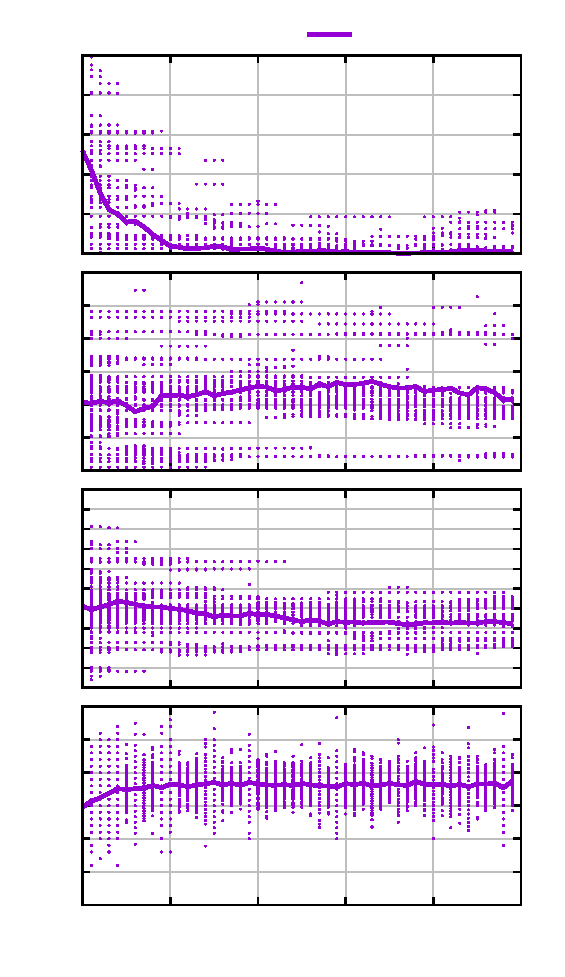
\includegraphics{pictures/top_optimization}}%
    \gplfronttext
  \end{picture}%
\endgroup
